\chapter{Bedürfnisanalyse}
Im Kapitel der Bedürfnisanalyse werden Anwendungsfälle ermittelt, welche mit Smartwatches abgedeckt werden können. Zusätzlich wird eine grobe Bedarfsanalyse für Applikationen durchgeführt, welche in Verbindung zur siot.net-Plattform stehen.

\section{Smartwatch Applikationen}
\subsection{Gesundheit}
Im Gesundheitssektor gibt es einige Anwendungsfälle, welche mit einer smarten Uhr abgedeckt werden können.

Eine Smartwatch bietet die Möglichkeit, sich überwachen zu lassen. Da die Computeruhr mit vielen Sensoren, wie z.B. Bewegungssensor oder Herzfrequenzmesser ausgerüstet ist, hat sie die Möglichkeit, den Träger sehr genau zu analysieren.

Ein Sturz des Benutzers kann durch die Auswertung der Sensormessdaten erkennt werden. Dies kann genutzt werden um einen Benachrichtigungen an Personen oder Systeme auszulösen, welche diese Informationen empfangen dürfen. Um nicht jede Ungereimtheit zu melden, sollte ein Zwischenschritt vorhanden sein. Den Träger mit taktilen und optischen Signalen aufmerksam machen, dass ein Gesundheitsbericht gesendet wird. Falls keine Reaktion erfolgt, kann ein Alarm an Vertrauenspersonen oder bei schwerwiegenden Bedrohungen gleich ein Notruf ausgelöst werden. Dieser Notruf kann mit wichtigen Daten angereichert werden, wie z.B. aktuelle Pulsdaten, die \gls{GPS} Koordinaten und Gesundheitskarte des Patienten. Der Sturz ist nur ein Beispiel, dieser Anwendungsfall kann für weitere Gesundheitsgefährdende Lebenslagen verwendet werden.

Ein weiterer nützlicher Use-Case ist, Alarme von Patienten im Spital. Hier kann das Pflegepersonal mit Smartwatches, Patientenalarme erhalten. Die Alarme sollten möglichst nur Pfleger/innen erhalten, welche sich in der Nähe des Patienten aufhalten. Wenn mehrere Pfleger/innen benachrichtigt werden, kann eine Pflegeperson den Alarm bestätigen und die Verantwortung für den Patienten übernehmen. Dies verkürzt die Reaktionszeit und vermeidet Doppelspurigkeiten.

\subsection{Smart Home}
Für die Fernbedienung von Geräten im Haus oder Wohnung eignet sich die Smartwatch gut. Mit eingebautem Touchscreen und Vibrationsmotor, haben die kleinen Handgelenkrechner die Möglichkeit, Informationen visuell wie auch taktil an die Person zu bringen.

Geräte im Haushalt können überwacht werden. Dies hilft Gefahren abzuwenden. Wenn eine Herdplatte noch läuft, kann ein Alarm ausgelöst werden und es kann gleich mit der Uhr die Platte ausgeschalten werden.

Die Funktion, das Licht vom Handgelenk aus zu bedienen, bietet für jeden einen Mehrwert. Es ist bequem das Licht im Zimmer mit dem Touchscreen ein- und auszuschalten. Weiterhin können auch virtuelle Dimmer eingesetzt und Zeitsteuerung bedient werden. Auch eine automatische Beleuchtung, durch erkennen der Helligkeit im Raum, ist eine Funktion mit hohem Potenzial.

Eine weitere Anwendungsmöglichkeit besteht bei der Waschmaschine. Die Restzeit des Waschgangs kann auf dem Bildschirm angezeigt werden. Wenn der Waschgang beendet ist, wird der Träger mit einer Nachricht notifiziert.

Des Weiteren ist das Fernbedienen von allen Multimediageräten übers Handgelenk sehr praktisch. Es genügt eine Uhr und braucht somit keine verschiedenen proprietären Steuerungen. Dies wird heute bereits mit Smartphone Apps praktiziert. Durch die Sprachsteuerung können Personen mit einer Leseschwäche die Uhr verwenden ohne die Lesebrille aufzusuchen.

\subsection{Sport}
Heute werden Smartwatches hauptsächlich als Fitnesstracker verwendet (vgl. \cite{eres:stsw}}. Das Praktische an den Uhren unter den Wearables ist, dass diese nicht nur für zum Sport treiben genutzt werden kann. Hier erhält der Endkunde ein Gerät für den Alltag und die Freizeit.

Im Sportbereich können mit den vorhandenen Sensoren viele verschiedene Werte ermittelt und analysiert werden. Mit den nötigen Voreinstellungen, wie Körpermasse, Schrittlänge, Alter und Geschlecht, ist es möglich, Bewegungsdaten genau aufzuzeichnen. Mit den Daten können für den Anwender interessante Informationen berechnet werden. Für Hobbysportler meist relevante Berechnungen sind Zeit, Schritte, Geschwindigkeit und Kalorienverbrauch. Erfahrene Sportler verbessern ihre Fähigkeiten, durch betrachten von Auswertungen der Körperbelastungen, z.B. Beschleunigung, Stärke, Drehmoment und weitere.

\subsection{Ortsbezogen}
Applikationen, welche umgebungsorientiert arbeiten, sind geeignete Kandidaten für Smartwatches. Durch die permanente Anzeige am Handgelenk, können schnell ändernde Daten dauerhaft im Auge behalten werden.

Ein Punkt ist Geofencing. Mit Geofencing werden automatische Aktionen eingeleitet. Diese geschehen, sobald bestimmte geografische Grenzen überschritten werden. Über eine Ortung des Gerätes kann ermittelt werden, ob sich dieses in einer Geofencing Zone befindet. Mit Smartwatches kann dies effektive genutzt werden, da durch den immer sichtbaren Bildschirm, die ortsrelevanten Daten ohne Zeitverlust verfügbar gemacht werden.\\
Eine Geofencing Anwendung könnte unteranderem Sehenswürdigkeiten präsentieren. Eine App, welche für jede Sehenswürdigkeit eine Geofencing Zone errichtet oder kennt und jeweils die Auskunft des Objektes darstellt.\\
Ein Anwendungsfall dazu ist auch, das Smartphone zu überwachen. Die Uhr kann den Träger informieren, wenn sich die Geofencingzonen, welche sich beide errichten durch ihre Sende- und Empfangsleistung, nicht mehr überschneiden. Wobei hier die geografischen Daten irrelevant sind.

Die gleiche Methode bietet sich an, Personen mit Smartwatches in der Nähe zu scannen. Diese Funktion kann bei Partnervermittlungsapplikationen effektiv eingesetzt werden. Durch den vorhandenen Touchscreen können potenzielle Datingpartner angezeigt und kontaktiert werden. In der schnelllebigen Welt sind sich schnell erschliessende Kontakte sehr willkommen.

Die Indoornavigation ist ein Bedürfnis, welches mit Smartwatches nicht gelöst, jedoch eine Erweiterung sein kann. In Zusammenarbeit mit Beacons/Eddystones und/oder Access Points können die Standorte von Smartwatchträgern, im inneren von Räumen, ermittelt werden. Beacons und Eddystones sind Sender/Empfänger, die per Bluetooth Low Energy (\gls{BLE}, Bluetooth 4.0 oder  Bluetooth Smart) Informationen aussenden.\\
Grossfirmen könnten einen grossen Nutzen aus dieser Technologiekombination schöpfen. Die Mitarbeiter dürften ihren Standort preisgeben, damit diese auf einer digitalen Gebäudekarte angezeigt werden können. Es würde die Effizienz erhöhen. Es können Geofencing Zonen definiert werden, um die Zeiterfassung zu automatisieren. Beim eintretten, des geografisch definierten Bereichs, welcher zu Arbeitszone gehört, wird Arbeitszeit erfasst. Verlässt der Mitarbeiter diesen Teil des Gebäudes, wird die Arbeitszeiterfassung gestoppt.\\
Zusätzlich kann das Problem mit den Shared-Desk Arbeitsplätzen gelöst werden. Bei diesem Arbeitsplatzmodell haben die Mitarbeiter keinen festen Arbeitsplatz. Es muss jeden Tag ein neuer aufgesucht werden. Um keine unnötige Zeit beim Aufsuchen zu verlieren, kann sich der Angestellte, mit einer Smartwatch ausgestattet, anzeigen lassen ob in einem Bereich ein freier Platz ist. Und beim erreichen des Schreibtisches kann dieser sich mit der Watch anmelden und den Platz als besetzt markieren.
\newpage

\subsection{Authentifikation}
Im Authentifikationssektor gibt es einige Bedürfnisse, welche mit Smartwatches gedeckt werden können.

Mit der Smartwatch Türen entriegeln, ist ein geeigneter Anwendungsfall. Heute benutzen die meisten Automobilhersteller ein Keyless System für ihre Fahrzeuge. Mit diesen Systemen hat der Fahrer ein Sender/Empfänger als Schlüssel, mit einem einzigartigen Zertifikat, welches sich mit jenem im Fahrzeug korreliert. Türen werden geöffnet und Motoren werden gestartet. Diese Funktionen könnte auch die Smartwatch übernehmen. Damit hätte der Fahrzeugbesitzer ein Utensil weniger mit sich zu tragen.

Die intelligente Uhr hat das Potenzial, Personalausweise zu ersetzen. Wie bereits im vorherigen Abschnitt - Ortsbezogen - erwähnt, kann es zur Zeiterfassung genutzt werden. Das heisst, Angestellte können sich damit auch ausweisen.

\subsection{Finanztechnologie - FinTech}
Die Möglichkeit zu haben, mit der Uhr Zahlungen zu autorisieren, ist ein Bedürfnis, welches erschaffen werden kann. Denn es scheint praktisch zu sein, einkaufen zu gehen ohne das Portemonnaie dabei zu haben. Es sind Lösungen vorhanden, welche mit Smartphones funktionieren {(Abbildung 4.1 Apple Pay/Google Wallet/TWINT)}. Mit der Lancierung der Apple Watch, erreichte die erste Smartwatch mit einer Zahlfunktion (sie unterstützt Apple Pay) den Markt.
\begin{figure}[H]
  \centering
  \includegraphics[scale=0.2]{98_Bilder/04_Anwendungen/APay_GWallet_PFTwint.png}
  \caption[Mobile Zahlungslösungen: Apple Pay, Google Wallet und TWINT powered by PostFinance]{Bekannte Zahlungslösungen für Smartphones: Apple Pay, Google Wallet und TWINT powered by PostFinance}
  \footnotesize \url{http://www.apple.com/apple-pay/} \url{https://wallet.google.com/} \url{http://www.twint.ch/ueber_uns/medien/}, 04.12.2015
\end{figure}

\section{Smartwatch Applikationen für siot.net}
Die siot.net-Plattform bietet sich bestens als Kommunikationsschnittstelle für die Applikationen an, welche im vorherigen Abschnitt ermittelt wurden. Die meisten Bedürfnisse verlangen irgendeine Art von Kommunikation. Ob es nur übermitteln der Sensordaten ist oder die Abfrage eines Sicherheitstokens ist. Die siot.net-Plattform erlaubt sämtliche Informationen über ihre Schnittstelle auszutauschen. Smartphones und Smartwatches sind ideale "`Things"' für \gls{IoT}-Anwendungen. Mit der Anbindung an die siot.net-Plattform kann jede beliebige \gls{IoT}-Applikation von den Daten dieser Geräte Nutzen erzielen.

\subsection{siot.net Gateway Library}
Um Verknüpfungen individueller Applikationen von Smartwatches oder Smartphones mit der Plattform zu ermöglichen, sollte es eine generische Bibliothek geben.
Diese sollte eine einfache Schnittstelle implementieren, welche Applikation an die siot.net-Plattform anbindet. Dies erleichtert ein Smartphone oder eine Smartwatch als ein "`Thing"' in das \gls{IoT} zu integrieren. Die Daten welche gesendet werden sollen, hängt vom Nutzen der Applikation ab. Dies hat jeder Entwickler selber zu definieren. Somit soll das gesamte Potzenzial eines Android Gerätes augenutzt werden können.
Zusätzlich vereinfacht die automatische Erkennung aller Sensoren und Vorbereitung ihrer Konfigurationsdaten die Entwicklung von Apps, welche Messwerte ans siot.net kommunizieren wollen.

\subsection{siot.net Sensorcenter}
Jedes Android Gerät kann mit den eingebauten Sensoren hervorragend als Sensorstation dienen. Um die Vielzahl von Sensoren in Eigenregie zum siot.net zu manifestieren und Sensordaten preiszugeben, sollte es eine App geben, mit einer leicht verständlichen, grafischen Benutzeroberfläche.

\subsection{siot.net Dashboard App}
Um eine Auswertung und Darstellung von den Daten zu erhalten, gibt es bereits eine Dashboard Webapplikation (siot.io). Um diese Funktionen einem Smartphone, in einer kompakten Form, zur Verfügung zu stellen, eignet sich eine App. Diese App sollte von Vorteil durch den Benutzer konfigurierbar sein.

\subsection{Herzfrequenzüberwachung}
Personen, welche ihren Puls im Griff haben wollen, leichte gesundheitliche Probleme haben oder bei Unregelmässigkeiten der Herzfrequenz jemanden alarmieren wollen, würden eine Herzfrequenzüberwachung begrüssen. Diese Anwendungsfälle können mit einer Smartwatch, mit Pulsmesser, und der siot.net-Plattform abgedeckt werden.

\subsection{Steuerung von Modellen}
Modellbau spielt eine grosse Rolle im Bereich des Internet of Things. Es gibt viele Forschungsprojekte, welche mit Hilfe von Drohnen durchgeführt werden. Darum ist die Kombination von Modellbau und Smartphones keine Weltneuheit. Es wird schon rege verwendet, wie bei der Parrot bebop Drohne (siehe Abbildung 4.2). Das Potenzial, mit einer Steuerung (Smartphone oder Smartwatch). Mehrere Modelle simultan zu steuern, scheint jedoch noch nicht im grossen Stile abgerufen zu werden. Mit der Einbindung von Modellen ins Internet der Dinge, zusätzlich gekoppelt mit einer smarten Steuerungseinheit, kann dieses Bedürfnis abgedeckt werden. Die siot.net Umgebung bietet dazu eine günstige Ausgangslage.
\begin{figure}[h]
  \centering
  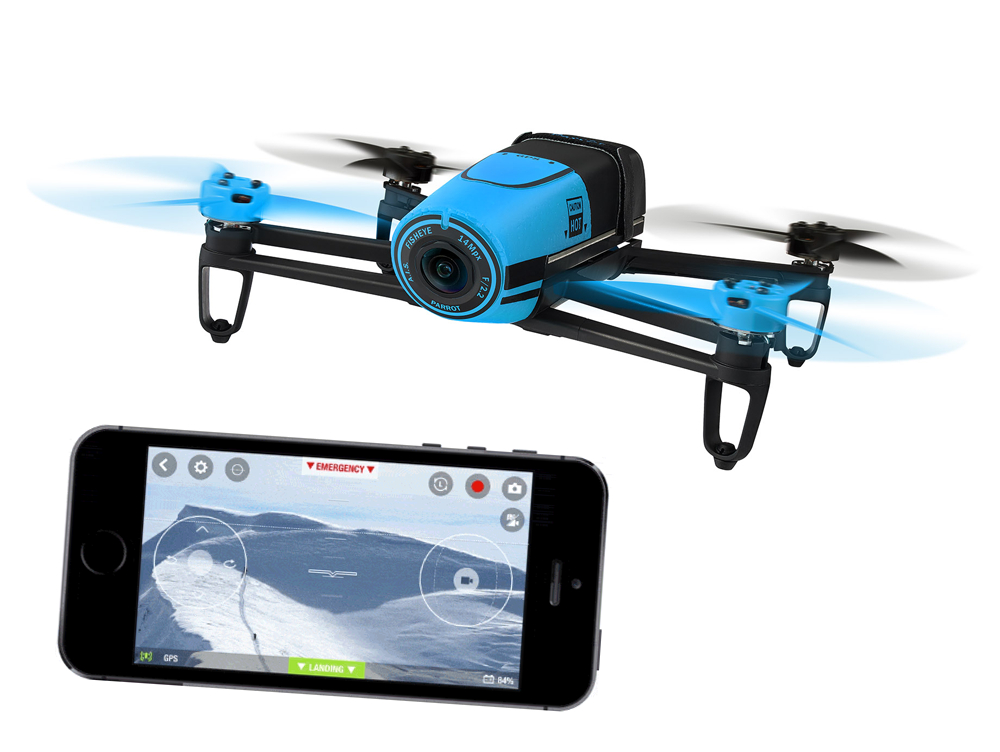
\includegraphics[scale=1]{98_Bilder/04_Anwendungen/parrotdrone}
  \caption[Smartphone gesteuerte Drohne: Parrot bebop]{Parrot bietet Drohnen an, welche mit dem Smartphone gesteuert werden können: Parrot bebop}
  \footnotesize \url{https://s.gravis.de/p/z1/parrot-bebop-drone-kamera-drohne-fuer-smartphones-tablets-gps-blau_z1.jpg}, 04.12.2015
\end{figure}
